\documentclass[CAT]{TFUOC}%IB: CASTELLÀ, CAT: CATALÀ, ENG: ANGLÈS

%Introducció de dades del treball
\title{Títol del treball complet i tan llarg com sigui necessari}
\titcrt{Títol molt curt} %Títol curt que apareixerà a la capçalera
\author{Nom Estudiant Estudiant}
\date{21 de setembre de 2021}


\nomPDC{Nom Tutor Tutora}
\nomPRA{Nomeni Professorat Responsable}
\titulac{Màster en XXX}
\area{Àrea del treball}
\idioma{Català}
\credits{15}
\parcla{paraula, clau, treball}

\licenc{ccBy}
%Possibles llicències
%ccByNcNd
%ccByNcSa
%ccByNc
%ccByNd
%ccBySa
%ccBy
%GNU
%copyright


%%%%%%%%%%
% Resum en l'idioma

\abstractidioma{
Màxim 250 paraules, amb la finalitat, context d’aplicació, metodologia, resultats i conclusions del treball.
}

% Resum en anglès.
\abstractenglish{
A maximum of 250 words, detailing the purpose, context of application, methodology, results and conclusions of the work.
}

\begin{document}

\estructura

\tableofcontents

\listoffigures

\listoftables




\chapter{Introducció}

Aquesta plantilla es concep com una guia per a l’estudiant. Es pot adaptar a les necessitats de cada treball, sempre que el/la tutor/a del treball hi estigui d’acord.

\section{Context i justificació del treball}


Punt de partida del treball (Quina és la necessitat a cobrir? Per què és un tema rellevant? Com es resol el problema de moment?) i aportació realitzada (Quin resultat es vol obtenir?).

És important tenir en compte que el treball final ha de ser comprensible per a qualsevol persona que conegui l'àrea de coneixement, però no té perquè ser experta en el tema del que versa el treball.

\section{Objectius del treball}

Llistat dels objectius del treball.

\section{Impacte en sostenibilitat, ètic-social i de diversitat}
\label{s:etic}

Aquesta secció hauria d'identificar els impactes positius i/o negatius del treball final en les tres dimensions de la competència transversal UOC “Compromís ètic i global”.
 
La Guia transversal sobre la Competència Ètica i Global us ajudarà a redactar aquests apartats.


\section{Enfocament i mètode seguit}

Menció de quines són les possibles estratègies per dur a terme el treball i quina és l’estratègia triada (desenvolupar un producte nou, adaptar un producte existent…). Cal incloure una valoració de per què aquesta és l’estratègia més apropiada per aconseguir els objectius.   	



\section{Planificació del treball}

Descripció dels recursos necessaris per fer el treball, les tasques a realitzar i una planificació temporal de cada tasca mitjançant un diagrama de Gantt o similar. Aquesta planificació hauria de marcar quins són les fites parcials de cadascuna de les PAC.



\section{Breu sumari de productes obtinguts}

No cal entrar en detall: la descripció detallada es farà a la resta de capítols.

%No és necessari entrar detalladament: la descripció detallada es farà en la resta de capítols.

\section{Breu descripció dels altres capítols de la memòria}

Breu explicació dels continguts de cada capítol i la seva relació amb el projecte global.

%\chapter{Estat de l'art}

%Estat de l'art del tema en qüestió. Hauria d'acabar mostrant per què el treball és important i aporta alguna cosa, i amb les hipòtesis del treball.

\chapter{Materials i mètodes}
En aquests apartats, cal descriure:
\begin{itemize}
    \item Els aspectes més rellevant del disseny i desenvolupament del treball.
    \item La metodologia triada per a fer aquest desenvolupament, descrivint les alternatives possibles, les decisions preses, i els criteris utilitzats per prendre aquestes decisions.
    \item Els productes obtinguts.
\end{itemize}

 
\textbf{L’estructuració dels capítols pot variar segons el tipus de treball.}  
 
En cas que s’escaigui, s’inclourà un apartat de “Valoració econòmica del treball”. Aquest apartat indicarà les despeses associades al desenvolupament i manteniment del treball, així com els beneficis econòmics obtinguts i una anàlisi final sobre la viabilitat del producte.



\chapter{Resultats}

Detalleu en aquest apartat els resultats obtinguts utilitzant la metodologia descrita a l’apartat anterior.


%Recull dels resultats del treball. Hauria d'haver-hi una correspondència amb la metodologia en el sentit que els resultats és el que s'obté després d'haver aplicat la metodologia.

Les figures han d'estar explicades i citades en el text, com la \ref{fig:my_label}, en la qual es mostra l'error en funció de la distància, en unitats arbitràries. A totes les gràfiques ha d'haver el títol dels eixos.

\begin{figure}[!htbp]
    \centering
    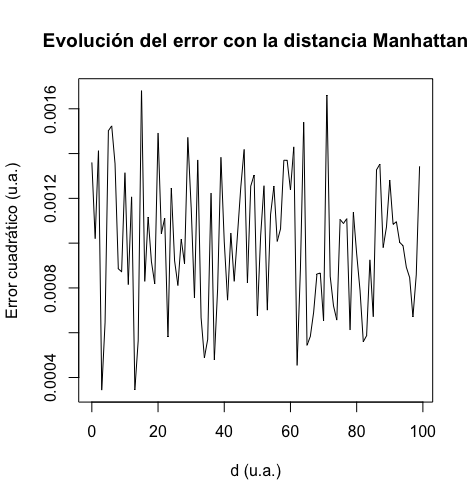
\includegraphics[width=7truecm]{Rplotmanh.png}
    \caption{Error en funcio de la distància en unitats arbitràries.}
    \label{fig:my_label}
\end{figure}

%\chapter{Discussió}
%Discussió dels resultats en el context del projecte. És en aquest apartat on cobren sentit i en el qual es responen les preguntes de recerca i es mostra com els resultats donen resposta als problemes plantejats.

%Aquesta part pot ser que no apliqui segons el tipus de treball.

%\chapter{Valoració econòmica}
%En cas que correspongui, s'inclourà un apartat de ``Valoració econòmica del treball". Aquest apartat indicarà les despeses associades al desenvolupament i manteniment del treball, així com els beneficis econòmics obtinguts. Cal fer una anàlisi final sobre la viabilitat del producte.

\chapter{Conclusions i treballs futurs}

%\section{Conclusions}
Aquest capítol ha d'incloure:
\begin{itemize}
\item Una descripció de les conclusions del treball:
\begin{itemize}
    \item Un cop s’han obtingut els resultats quines conclusions s’extreu?
    \item Aquests resultats són els esperats? O han estat sorprenents? Per què?
\end{itemize}
\item Una reflexió crítica sobre l’assoliment dels objectius plantejats inicialment:
\begin{itemize}
    \item Hem assolit tots els objectius? Si la resposta és negativa, per quin motiu?
\end{itemize}
\item Una anàlisi crítica del seguiment de la planificació i metodologia al llarg del producte:
\begin{itemize}
    \item S’ha seguit la planificació?
    \item La metodología prevista ha estat prou adequada?
    \item Ha calgut introduir canvis per garantir l’èxit del treball? Per què?
\end{itemize}
\item Dels impactes previstos a \ref{s:etic}, ètic-socials, de sostenibilitat i de diversitat, avaluaeu/esmenteu si s'han mitigat (si eren negatius) o si s'han aconseguit (si eren positius). 
\item Si han aparegut impactes no previstos a \ref{s:etic}, avaluar/esmentar com s'han mitigat (si eren negatius) o què han aportat (si eren positius).
\item Les línies de treball futur que no s’han pogut explorar en aquest treball i han quedat pendents.


%\item Una descripció de les conclusions del treball: Quines lliçons s'han après del treball?
%\item Una reflexió crítica sobre l'assoliment dels objectius plantejats inicialment: Hem aconseguit tots els objectius? Si la resposta és negativa, per quin motiu?
%\item Dels impactes previstos a la secció \ref{s:etic}, una avaluació, o almenys, esment, sobre si s'han mitigat (si eren negatius) o si s'han aconseguit (si eren positius). 
\end{itemize}

%\section{Línies de futur}
%Les línies de treball futur que no s'han pogut explorar en aquest treball i han quedat pendents.

%\section{Seguiment de la planificació}
%Una anàlisi crítica del seguiment de la planificació i metodologia al llarg del treball: 
%\begin{itemize}
%    \item  S'ha seguit la planificació? 
%    \item La metodologia prevista ha estat l'adequada? 
%    \item Ha calgut introduir canvis per garantir l'èxit del treball? Per què?
%\end{itemize}

\chapter{Glossari}

Definició dels termes i acrònims més rellevants utilitzats dins la Memòria.

%Definició dels termes i acrònims més rellevants utilitzats dins de la Memòria.

\chapter{Bibliografia}

Llista numerada de les referències bibliogràfiques utilitzades dins de la memòria. En cada lloc on s'utilitzi una referència dins del text, s'ha d'indicar citant el número de la referència, per exemple: [7].

És molt important incloure totes les referències utilitzades i citar-les apropiadament, és a dir, incloent tota la informació necessària per identificar la referència. La informació mínima que s'ha d'incloure segons el tipus de referència és:

\begin{itemize}
\item Llibre: Autors, Títol, Edició (si escau) Editorial, Ciutat, Any.
\item  Article de revista: Autors, Títol, Nom de la Revista, Número de Pàgina inicial i final, Número de la revesteixi / Volum, Any.
\item  Web: URL i data en què s'ha visitat.
\end{itemize}

Informació de com citar documents: \url{http://biblioteca.uoc.edu/es/recursos/citacion-bibliografica}.


\newpage
\appendix
Llistat d’apartats que són massa extensos per incloure dins la memòria i tenen un caràcter autocontingut (per exemple, manuals d’usuari, manuals d’instal·lació, etc.)
 
Depenent del tipus de treball, és possible que no calgui afegir cap annex.

\end{document}
